% ---------------------------------------------------------------------------
% Appendix: Model and Temperature Ablations
% Source: writeup/contents/appendix.tex:238-328
% Fixes applied per plan §5: temperature text rewritten to match its own table
%   (§5.9); significance stars vs reconstructed humans removed (§5.8);
%   "Claude Sonnet 3.5" -> Claude 3.5 Haiku with config-verified footnote (§5.2);
%   Llama-3-8B as capability floor (§5.1). Frontier tier rewritten from
%   results/merged_ranking/auction_cells.csv + auction_cells_summary.md:
%   the old gpt-5-mini column was sourced to misattributed GPT-4o logs
%   (recovered_logs/experiment_logs_with_explanation/V10) and is removed.
%   2026-07-10: added tab:gemma-fidelity (E4) and tab:frontier-grid (the
%   10-cell lever grid on 4 frontier models: gpt-5-mini/gpt-5/claude-sonnet-5/
%   gemini-2.5-flash), all recomputed from results/merged_ranking/auction_cells.csv.
% ---------------------------------------------------------------------------
\section{Model and Temperature Ablations}\label{app:ablations}

This appendix reports the stability ablations referenced in Section~\ref{sec:validation}---varying the sampling temperature of the GPT-4o anchor, and varying the base model on the seven-format fidelity battery---together with a corrected accounting of the frontier tier (four reasoning models: gpt-5-mini, gpt-5, claude-sonnet-5, gemini-2.5-flash). Throughout, the human column is the moment-matched reconstruction of Section~\ref{sec:reconstruction}; consistent with the epistemic policy stated there, we report \emph{no} significance tests against reconstructed human benchmarks, because such tests would treat a model-based reconstruction as if it were sampled micro-data. Comparisons to the human column should be read qualitatively---rankings, directions, and orders of magnitude. \TODO{Attach Monte-Carlo percentile bands (and, once available, the parametric-bootstrap bands of Appendix~\ref{app:human}) to the human column in both tables (plan \S 5.8).}

\subsection{Varying temperature for the GPT-4o agent}

We vary GPT-4o's sampling temperature $T \in \{0.1, 0.5, 1.0\}$ across the seven fidelity-battery formats (Table~\ref{tab:temperature}; Figure~\ref{fig:ablations-temperature}). The temperature parameter controls the randomness of the model's outputs, with lower values producing more deterministic responses and higher values introducing more variability.

Two facts stand out. First, temperature effects are modest and, crucially, \emph{non-monotonic}: no temperature setting dominates. $T=0.1$ is strictly best in three of the seven formats (both ascending-clock formats and FPSB-CV) and strictly worst in three others (SPSB-IPV, SPSB-APV, and FPSB-IPV), with the remaining format (SPSB-CV) ordered $T=1.0 < T=0.1 < T=0.5$. Second, the pattern is consistent with temperature scaling the dispersion around the model's modal action rather than changing the underlying strategy: at $T=0.1$ the clock formats become exactly truthful (SMAD $= 0.00$) because near-deterministic decoding removes stochastic exits from an already-truthful modal policy, while in the sealed-bid formats the same determinism locks in the modal bias. We therefore retain $T=0.5$ throughout the paper as a \emph{convention}---it is the most common setting in LLM-based simulation \citep{horton2023large} and preserves comparability across models and with prior work---not because it is performance-optimal in any particular format. Temperature reappears in Section~\ref{sec:humans} as a candidate knob for \emph{cardinal} calibration to human levels; its effects there are likewise non-monotonic (on the rebuilt grid's normalization, SPSB-IPV SMAD is $15.1/8.9/13.2$ at $T=0.1/0.5/1.0$).

\begin{figure}[H]
    \centering
    
\includegraphics[scale=0.35]{appendix2_temperature_comparison.png}
    \caption{Comparison of the bidding behavior of reconstructed human participants and GPT-4o across three temperature settings ($T=0.1, 0.5, 1.0$) in seven auction formats. The horizontal bars represent the scaled mean absolute deviation (SMAD) from the theoretical benchmark, with error bars indicating 95\% confidence intervals (for the LLM cells only; see the text of this appendix for the human column's epistemic status).}
    \label{fig:ablations-temperature}
\end{figure}

\begin{table}[htbp]
\centering
\begin{tabular}{l|ccc}
\hline
Auction Format & $T=0.1$ & $T=0.5$ & $T=1.0$ \\
\hline
AC-B (closed clock), APV & 0.00 & 0.47 & 2.15 \\
AC (open clock), APV & 0.00 & 0.81 & 1.00 \\
SPSB, IPV & 14.77 & 8.69 & 12.89 \\
SPSB, APV & 12.87 & 10.73 & 12.75 \\
FPSB, CV & 39.00 & 59.99 & 42.92 \\
SPSB, CV & 35.51 & 40.60 & 33.53 \\
FPSB, IPV & 28.07 & 27.55 & 24.99 \\
\hline
\end{tabular}
\caption{Temperature effects on GPT-4o bidding behavior (SMAD, \%). SMAD = scaled mean absolute deviation from the theoretical benchmark. No temperature dominates: $T=0.1$ is strictly best in three formats and strictly worst in three others. Values use the legacy figure normalization ($\mathbb{E}[b^\star]=25$); the rebuilt cell-level grid normalizes by $24.5$, making values uniformly $\approx 2\%$ larger (e.g., SPSB-IPV $15.1/8.9/13.2$)---orderings and the non-monotonicity are unaffected.}
\label{tab:temperature}
\end{table}

\subsection{Varying the base model}

We repeat the seven-format fidelity battery, holding prompts fixed and $T=0.5$, for three models beyond the GPT-4o anchor: Claude 3.5 Haiku, Gemini 2.0 Flash, and Llama-3-8B-Instruct (an open-weight model).\footnote{Model identifiers: \texttt{claude-3-5-haiku-20241022}, \texttt{gemini-2.0-flash}, \texttt{Meta-Llama-3-8B-Instruct}, and, in the frontier tier below, \texttt{gpt-5-mini}, \texttt{gpt-5}, \texttt{claude-sonnet-5}, and \texttt{gemini-2.5-flash}. An earlier draft referred to the Anthropic model as ``Claude Sonnet 3.5''; the experiment configurations confirm that the runs stored under directories named \texttt{claude\_sonnet} (e.g., \texttt{robustness\_logs/V10/*claude\_sonnet*}) were in fact executed with \texttt{claude-3-5-haiku-20241022} (config-verified: \texttt{configs/clock/01\_06\_ascending\_clock\_apv\_claude\_sonnet.yaml}). The gpt-5-mini API ignores the temperature parameter.} Claude 3.5 Haiku and Gemini 2.0 Flash belong to the canonical model set of Section~\ref{sec:design}; Llama-3-8B-Instruct and the frontier reasoning models of Section~\ref{app:ablations-frontier} (treated separately below, because their data coverage differs) bracket the canonical set from below and above. Results appear in Table~\ref{tab:models} and Figure~\ref{fig:ablations-models}. The fourth canonical model, Gemma 27B, ran a separate six-format sealed-bid fidelity battery (Table~\ref{tab:gemma-fidelity}); we report it apart from Table~\ref{tab:models} because its cells are recomputed from the cell-level dataset (\path{results/merged_ranking/auction_cells.csv}, normalizer $\mathbb{E}[b^\star]=24.5$), a normalization that differs from the legacy figure scaling of the Claude/Gemini/Llama columns here (the same $\approx\!2\%$ offset flagged for Table~\ref{tab:temperature}), so the columns are not directly comparable cell-for-cell.

Llama-3-8B-Instruct serves as the \emph{capability floor}. It exhibits substantially degraded performance across all auction formats (mean SMAD $= 57.58\%$), exceeding the reconstructed human benchmark in six of seven formats---evidence that open-weight availability at small scale is not sufficient for competent strategic play, and that the canonical models sit well inside the band where design levers have room to operate. Claude 3.5 Haiku and Gemini 2.0 Flash behave broadly like the GPT-4o anchor: near-truthful in the clock formats, moderate deviations in the sealed-bid formats, and large deviations under common values. \TODO{The SPSB-IPV cells will be recomputed on the harmonized canonical dataset alongside signed means (plan E8, \S 5.3); the Claude SMAD/signed-mean contrast (worse absolute, best signed) is expected to persist and will be reported as such.} \TODO{Regenerate the figure asset \texttt{appendix2\_model\_comparison.png}: the legend of the current PNG carries the superseded ``Claude Sonnet 3.5'' label (see footnote in this appendix), and its gpt-5-mini series rests on the misattributed logs documented in Section~\ref{app:ablations-frontier} of this appendix and must be dropped or rebuilt from the genuine cells.}

\paragraph{Gemma 27B and the difficulty ordering.} The open-weight Gemma 27B model ran the sealed-bid fidelity battery in six formats ($K=30$ per cell; Table~\ref{tab:gemma-fidelity}). Its mean SMAD is $19.09\%$, between the canonical models and the Llama floor. The more instructive fact is not the level but the \emph{shape}: Gemma does \emph{not} reproduce the human difficulty ordering cleanly. In the human data the first-price format is much harder than the second-price dominant-strategy format---FPSB-IPV SMAD $24.76\%$ versus SPSB-IPV $5.65\%$, a ratio of $4.4$---and GPT-4o preserves that ordering ($27.55\%/8.69\% = 3.2$). Gemma nearly flattens it: $24.80\%$ in FPSB-IPV against $19.88\%$ in SPSB-IPV, a ratio of only $1.25$. It deviates almost as much in the format where truthful bidding is a dominant strategy as in the format where equilibrium requires shading, so the fidelity ordering that the auction ranking exploits is, in part, model-specific rather than a universal property of LLM bidders. The two ascending-clock cells are not yet run for Gemma (the per-tick clock harness is prohibitively slow, and reconciling the survey-style elicitation with the tick protocol is deferred to the native-key runs), so the clock rows of Table~\ref{tab:models} have no Gemma entry. \TODO{Gemma ascending-clock (AC and AC-B) cells pending native-key runs; survey-vs-tick harmonization deferred.}

\begin{table}[htbp]
\centering
\footnotesize
\begin{tabular}{l c c}
\hline
Auction Format & SMAD vs.\ value (\%) & Signed mean dev.\ (\$) \\
\hline
FPSB, IPV & 24.80 & $-5.89$ \\
TPSB, IPV & 23.31 & $-5.45$ \\
SPSB, IPV & 19.88 & $-4.87$ \\
SPSB, APV & 18.67 & $-4.57$ \\
FPSB, CV & 16.08 & $-2.57$ \\
SPSB, CV & 11.80 & $-1.44$ \\
\hline
\end{tabular}
\caption{Gemma 27B sealed-bid fidelity battery (SMAD, \% of $\mathbb{E}[b^\star]=24.5$; signed mean deviation from value in dollars). Recomputed from \texttt{results/merged\_ranking/auction\_cells.csv} (group \texttt{gemma27b}, $K=30$ per cell). Mean SMAD across the six formats is $19.09\%$. Gemma's FPSB-IPV/SPSB-IPV ratio is $1.25$, against $4.4$ for reconstructed humans and $3.2$ for GPT-4o: the model does not reproduce the human difficulty ordering, so the fidelity ordering is partly model-specific. The two ascending-clock cells (AC, AC-B) were not run for Gemma (per-tick harness too slow; survey-vs-tick harmonization pending native-key runs). CV deviations are relative to the private signal and carry no dominant-strategy benchmark.}
\label{tab:gemma-fidelity}
\end{table}

\begin{figure}[H]
    \centering
    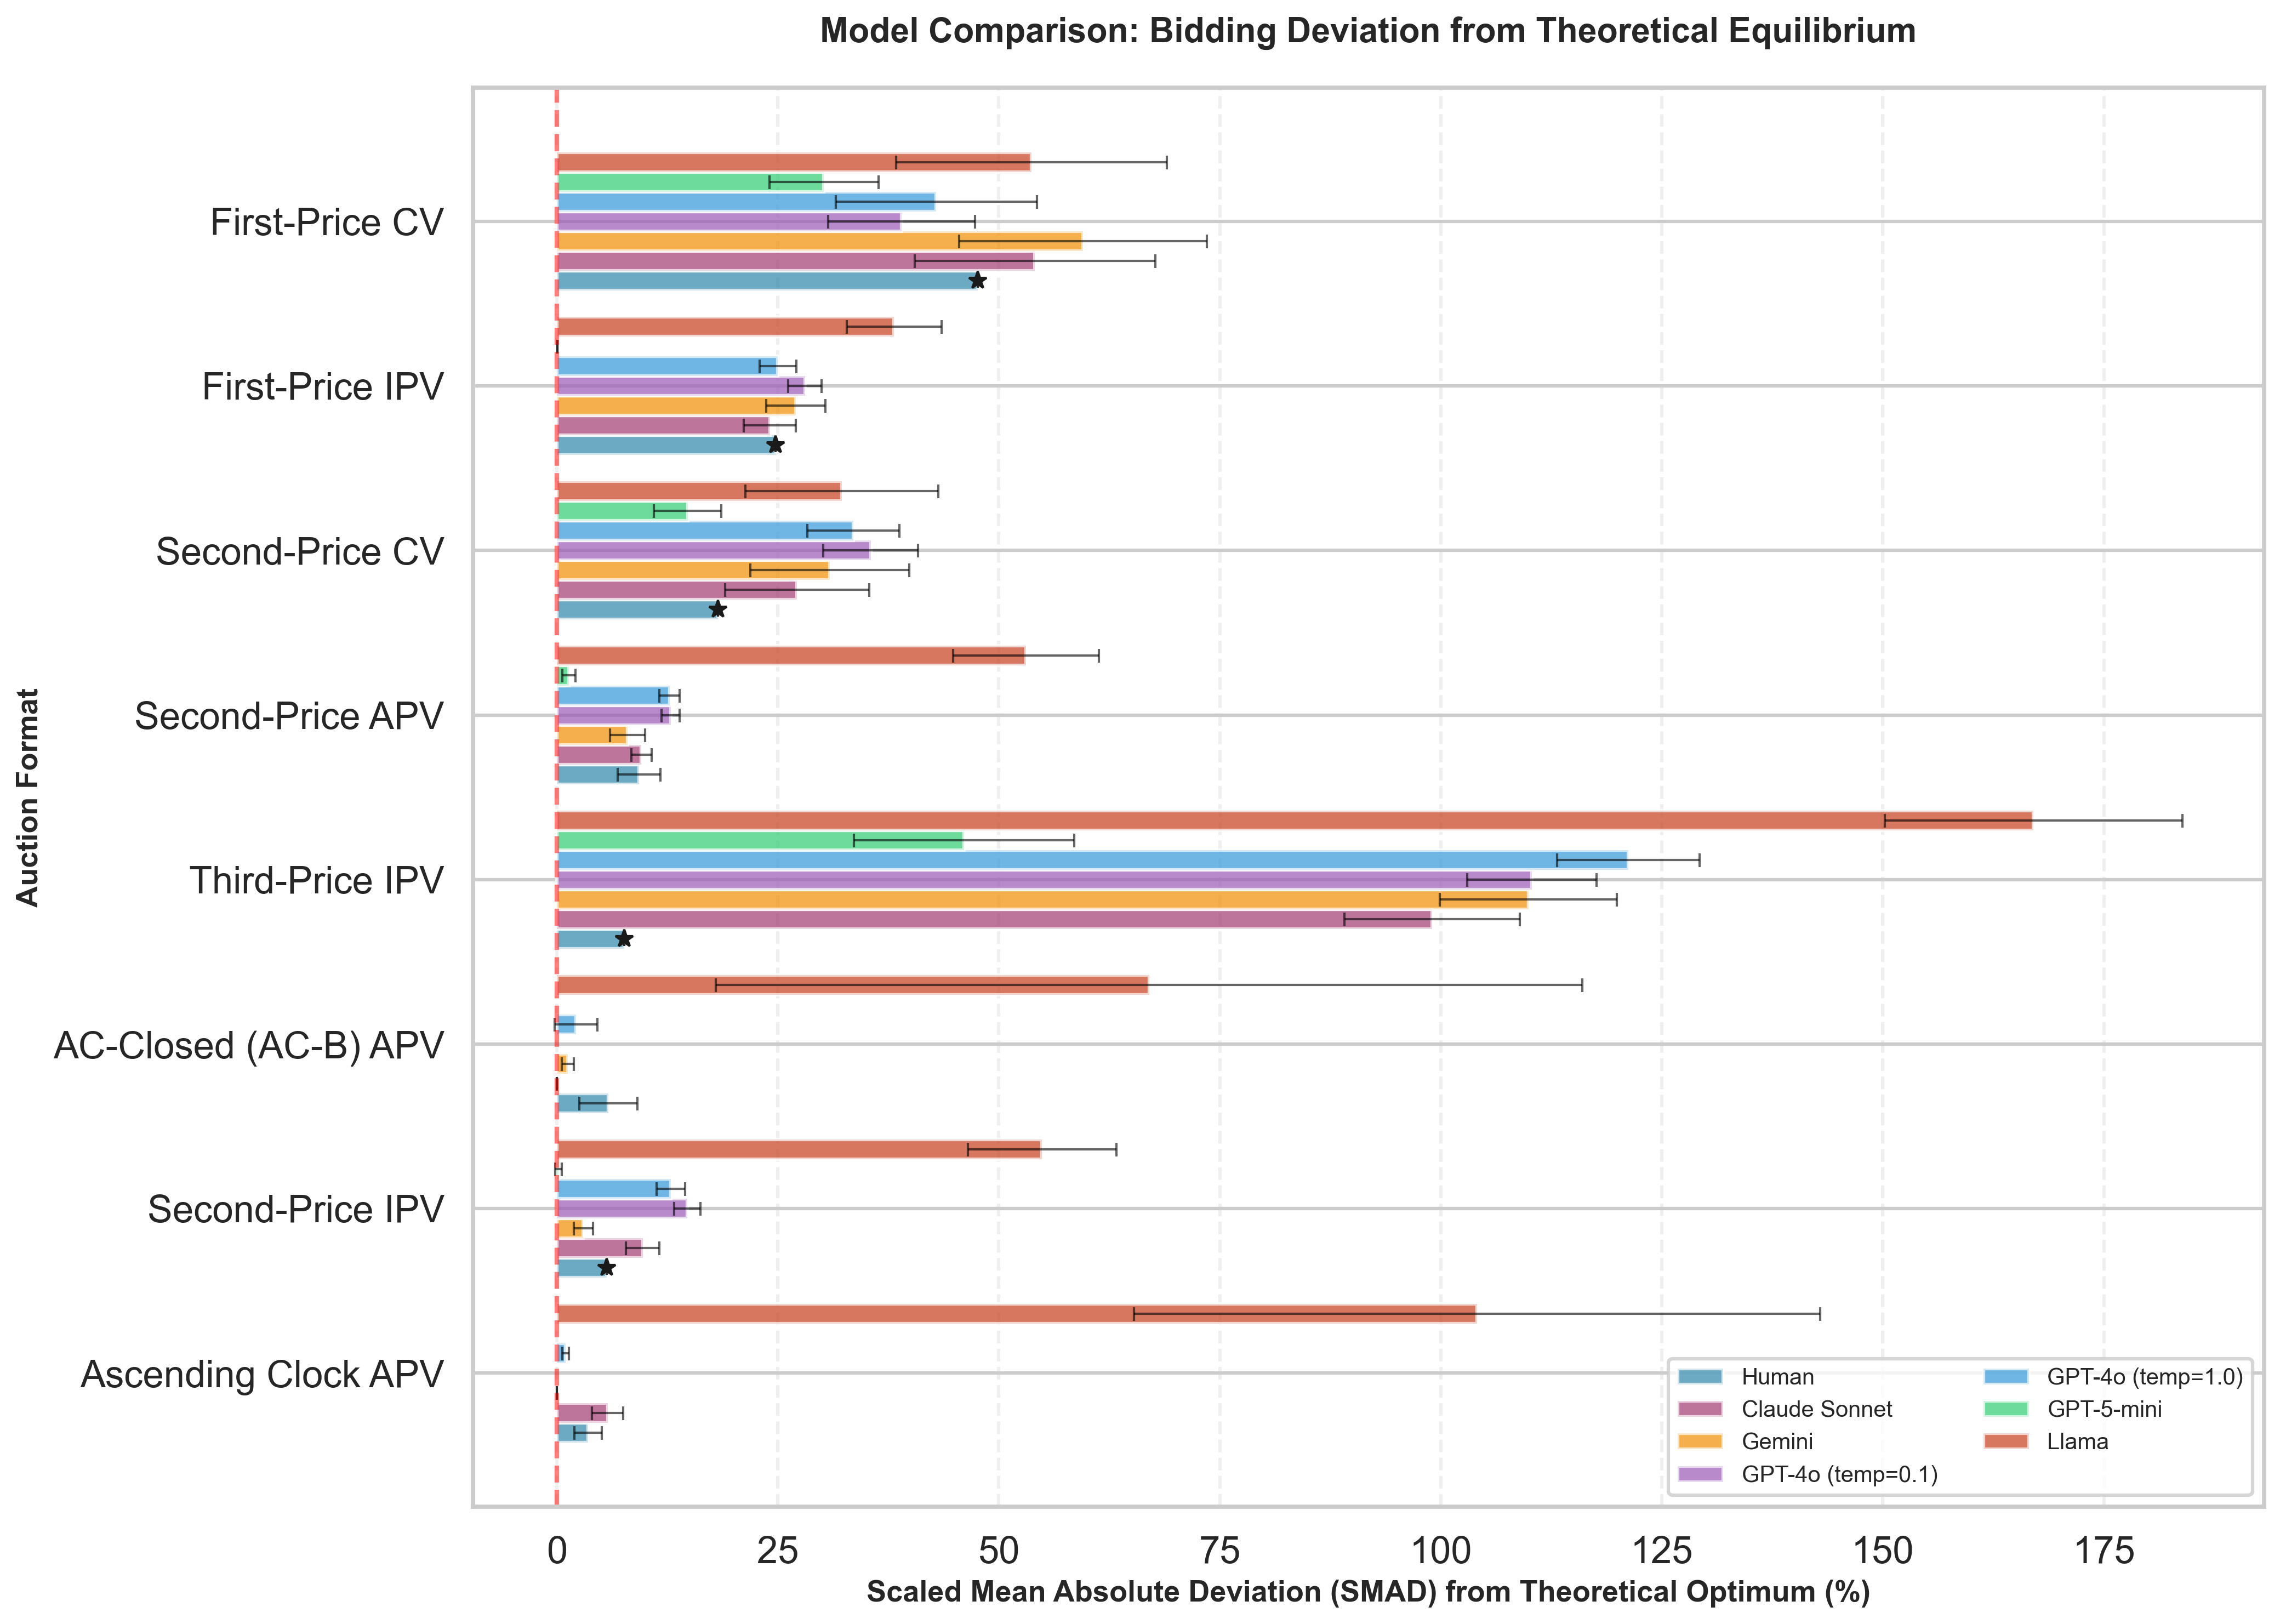
\includegraphics[scale=0.375]{appendix2_model_comparison.png}
    \caption{Comparison of the bidding behavior of reconstructed human participants and LLM agents across further foundation models in seven auction formats. The horizontal bars represent the scaled mean absolute deviation (SMAD) from the theoretical benchmark, with error bars indicating 95\% confidence intervals (LLM cells only). The gpt-5-mini series shown in the current asset is superseded (see the frontier discussion in the text; regeneration pending).}
    \label{fig:ablations-models}
\end{figure}

\begin{table}[htbp]
\centering
\begin{tabular}{l|c|ccc}
\hline
\multirow{2}{*}{Auction Format} & Human & Claude 3.5 & Gemini 2.0 & Llama-3-8B \\
 & (reconstr.) & Haiku & Flash & \\
\hline
FPSB, IPV & 24.76 & 24.09 & 27.05 & 38.16 \\
SPSB, IPV & 5.65 & 9.72 & 3.01 & 54.89 \\
AC-B (closed clock), APV & 5.83 & 0.00 & 1.26 & 67.00 \\
SPSB, APV & 9.31 & 9.58 & 8.02 & 53.08 \\
AC (open clock), APV & 3.54 & 5.74 & 0.00 & 104.10 \\
FPSB, CV & 47.59 & 54.07 & 59.50 & 53.68 \\
SPSB, CV & 18.23 & 27.19 & 30.89 & 32.27 \\
\hline
\end{tabular}
\caption{Fidelity battery across base models (SMAD, \%). SMAD = scaled mean absolute deviation from the theoretical benchmark. All models run at $T=0.5$. The human column is the moment-matched reconstruction of Section~\ref{sec:reconstruction}; no significance tests are reported against it because the reconstruction is model-based (see text and Appendix~\ref{app:human}). An earlier draft's gpt-5-mini column is removed: its source logs are GPT-4o (see the frontier subsection); the genuine gpt-5-mini cells appear in Table~\ref{tab:ablations-frontier}.}
\label{tab:models}
\end{table}

\subsection{The frontier tier: reasoning models do not uniformly dissolve the constraints}\label{app:ablations-frontier}

An earlier draft treated gpt-5-mini as a frontier \emph{ceiling} that plays near-optimally across a battery of sealed cells (mean SMAD $6.68\%$). That figure did not survive a provenance audit: the log tree from which it was computed (\path{recovered_logs/experiment_logs_with_explanation/V10/}) is GPT-4o in every run configuration---not gpt-5-mini---and shares most of its run identifiers with the anchor logs, so it is discarded. Two data sources now replace it. First, a genuine gpt-5-mini sealed-bid mechanism battery (Table~\ref{tab:ablations-frontier}), whose across-format mean SMAD \emph{against truthful value} is $19.09\%$ over the six robustness formats (or $16.6\%$ if the genuine clock cell below is included)---the $6.68\%$ figure is retired, not merely re-sourced. Second, and new to this draft, a full intervention grid run on four frontier models---gpt-5-mini, gpt-5, claude-sonnet-5, and gemini-2.5-flash (canonical identifiers; family \texttt{es\_v12} in \path{results/merged_ranking/auction_cells.csv})---which replaces the earlier claim that ``no gpt-5-mini intervention cells exist anywhere.'' The empty gpt-5-mini clock cells that motivated that claim are now explained: a configuration typo (\path{configs/clock/01_07_ascending_clock_apv_closed_gpt5mini.yaml} carried the invalid model id \texttt{gpt-4-mini}) suppressed the closed-clock robustness runs; with the typo fixed and the frontier battery's own \texttt{ascending\_clock\_closed} cell in hand ($K=50$, SMAD $1.25\%$), a genuine gpt-5-mini clock number exists and supersedes the empty cells.

\paragraph{The frontier intervention grid: truthful at baseline, but the backfire rungs retain teeth.} Table~\ref{tab:frontier-grid} reports the ten-cell lever grid across the four frontier models, entries recomputed from \path{auction_cells.csv} as mean deviation from value (dollars) with SMAD in parentheses. Three facts stand out. (i) \emph{All four frontier models are essentially exactly truthful at every sealed baseline}: mean deviations of $0.00$--$0.30$ and SMAD of $0$--$2.3\%$ across the sealed baseline cells, and the safety, payoff-tree, second-order-belief, and clock-framing description cells are inert (they land on the same $\approx\!0$ play, because there is no baseline error left to preserve). (ii) \emph{The menu restatement still breaks the frontier}, exactly the backfire the ranking predicts for its restatement rung: it moves claude-sonnet-5 catastrophically away from truthful play (mean deviation $-\$8.71$, SMAD $35.5\%$, $d=-3.8$, $p<10^{-58}$) and degrades gemini-2.5-flash (SMAD $2.3\% \to 9.1\%$, $p<10^{-8}$), while leaving gpt-5 and gpt-5-mini exactly truthful---the same sign-mixed, model-specific pattern the canonical menu cell shows, now with one model driven to a $35\%$ deviation. (iii) \emph{The true ascending clock makes frontier play \textbf{worse}, not better}: relative to their near-perfect sealed play, the closed clock raises claude-sonnet-5 from $0.27\%$ to $8.6\%$ SMAD and adds $+\$0.61$ (gpt-5) and $+\$0.28$ (gpt-5-mini) of mean deviation---an inversion of the canonical clock benefit, driven partly by the $\$0.5$-tick granularity of the clock grid interacting with models that otherwise bid value exactly. The extensive-form lever that helps bounded-rational agents is a small liability once the agent already plays the dominant strategy in the sealed format.

The gpt-5 cells carry reduced and uneven $K$: the model frequently omits the required response tags, and unparseable repetitions are dropped, so per-cell $n$ (in bids) ranges from $15$ to $150$ ($102$ for the SPSB baseline after its final top-up) (reported in Table~\ref{tab:frontier-grid}); the $n$ column should be read as a sample-size caveat; the run set is now frozen. gpt-5's DA cells were deliberately not run.

\TODO{gpt-5 intervention cells have reduced/uneven $K$ (15--150 parseable bids) from response-tag omissions; top up and re-freeze $n$ before the final draft. The frontier-battery runbook is \path{plan/FRONTIER_RUNBOOK.md}.}

The genuine cells sharpen, rather than remove, the paper's scope condition: \emph{frontier reasoning dissolves the bounded-rationality constraints where optimal play is textbook, and only there}. In the dominant-strategy format, gpt-5-mini is essentially perfect---mean deviation $-\$0.05$ (SMAD $0.2\%$) in SPSB-IPV and $-\$0.34$ ($1.4\%$) in SPSB-APV, truthful play at levels the canonical models reach only under the strongest levers. In FPSB-IPV, its bids sit $\$8.53$ below value on average, i.e., almost exactly on the risk-neutral equilibrium shading rule $\frac{n-1}{n}v$ (mean deviation from the RNE benchmark $+\$0.002$; SMAD against RNE $0.1\%$)---it applies the textbook formula.\footnote{The cell-level data (\path{results/merged_ranking/auction_cells.csv}) report deviations against both truthful bidding and each format's own equilibrium benchmark; against truthful bidding the FPSB cell reads SMAD $34.8\%$, which measures correct equilibrium shading, not error.} But in the \emph{third-price} format, where the equilibrium bid $\frac{n-1}{n-2}v$ exceeds value and no textbook formula is rehearsed in training corpora, the frontier model fails: with $n=3$ it overbids value by $+\$14.76$ on average yet remains $\$10.87$ \emph{below} the equilibrium bid $2v$ (SMAD $60.2\%$ against truthful play, $22.5\%$ against the equilibrium benchmark); with $n=5$ the same pattern appears at smaller scale ($+\$4.39$ above value, $\$4.11$ below the $\frac{4}{3}v$ equilibrium). It recognizes that third-price rules reward aggression but cannot compute how much. The common-value cells show similarly dispersed behavior (deviations relative to the private signal $-\$2.91$ and $-\$2.60$, with wide spreads; descriptive only, as no dominant-strategy benchmark exists).

The implication for the main text is a two-sided scope condition. On one side, at the frontier the gaps that the design levers close have vanished \emph{in the strategy-proof formats the ranking studies}---confirmed directly by the intervention grid of Table~\ref{tab:frontier-grid}, in which every safety, tree, and belief cell is inert because there is no baseline error left to preserve---which is why reasoning models are excluded from the main treatment grid, and why the ranking's practical relevance turns on deployed agent fleets occupying the sub-frontier regime for cost reasons (Section~\ref{sec:discussion}). On the other side, the third-price cells show that frontier reasoning does \emph{not} uniformly dissolve bounded rationality: where the required strategic computation is non-obvious, even the frontier model deviates by more than any canonical model deviates in second price. And the frontier grid shows that the backfire rungs keep their teeth: the menu restatement drives claude-sonnet-5 to a $35\%$ deviation and the true clock inverts into a small liability (Table~\ref{tab:frontier-grid}). Whether the levers of Section~\ref{sec:ranking} would repair a frontier model's third-price play---a format the grid does not yet cover---remains the natural next question.

\begin{table}[htbp]
\centering
\footnotesize
\begin{tabular}{l c c c c c}
\hline
Format & $n$ bids & Mean dev.\ vs.\ value (\$) & SMAD vs.\ $v$ (\%) & Mean dev.\ vs.\ $b^\star$ (\$) & SMAD vs.\ $b^\star$ (\%) \\
\hline
SPSB, IPV & 87 & $-0.05$ \([-0.15, 0.00]\) & 0.2 & $-0.05$ & 0.2 \\
SPSB, APV & 87 & $-0.34$ \([-0.53, -0.18]\) & 1.4 & $-0.34$ & 1.4 \\
FPSB, IPV & 87 & $-8.53$ \([-9.33, -7.74]\) & 34.8 & $+0.00$ & 0.1 \\
TPSB, IPV ($n{=}3$) & 87 & $+14.76$ \([12.32, 17.28]\) & 60.2 & $-10.87$ & 22.5 \\
TPSB, IPV ($n{=}5$) & 130 & $+4.39$ \([2.83, 6.19]\) & 26.5 & $-4.11$ & 18.2 \\
FPSB, CV & 90 & $-2.91$ \([-5.19, -0.74]\) & 36.6 & --- & --- \\
SPSB, CV & 90 & $-2.60$ \([-4.93, -0.37]\) & 36.9 & --- & --- \\
\hline
\end{tabular}
\caption{Genuine gpt-5-mini sealed-bid mechanism cells (\texttt{robustness\_logs/*\_gpt5mini}; brackets are bootstrap 95\% CIs on the mean deviation vs.\ value). $b^\star$ is each format's own benchmark: truthful bidding in SPSB, $\frac{n-1}{n}v$ in FPSB, $\frac{n-1}{n-2}v$ in TPSB. CV deviations are relative to the private signal and carry no dominant-strategy benchmark. The gpt-5-mini ascending-clock and intervention cells appear separately in Table~\ref{tab:frontier-grid} (frontier grid).}
\label{tab:ablations-frontier}
\end{table}

\begin{table}[htbp]
\centering
\footnotesize
\setlength{\tabcolsep}{4.5pt}
\begin{tabular}{ll cccc}
\toprule
& & \multicolumn{4}{c}{Mean dev.\ vs.\ value, \$ (SMAD vs.\ $v$, \%)} \\
\cmidrule(lr){3-6}
Lever grid cell & Family & gpt-5-mini & gpt-5$^{\dagger}$ & claude-sonnet-5 & gemini-2.5-flash \\
\midrule
\multicolumn{6}{l}{\emph{Sealed baselines}} \\
SPSB, IPV baseline & --- & $0.00$ ($0.0$) & $0.00$ ($0.0$; $n{=}102$) & $-0.07$ ($0.3$) & $-0.30$ ($2.3$) \\
Contingent baseline (axis 1) & --- & $0.00$ ($0.0$) & $0.00$ ($0.0$; $n{=}69$) & $0.00$ ($0.0$) & $-0.16$ ($0.9$) \\
Beliefs baseline (axis 3) & --- & $0.00$ ($0.0$) & $0.00$ ($0.0$; $n{=}45$) & $0.00$ ($0.0$) & $0.00$ ($0.2$) \\
\addlinespace
\multicolumn{6}{l}{\emph{Description / scaffold levers}} \\
Payoff Safety & B2 & $0.00$ ($0.0$) & $0.00$ ($0.0$; $n{=}132$) & $0.00$ ($0.0$) & $0.00$ ($0.0$) \\
Payoff Tree & C1 & $0.00$ ($0.0$) & $0.00$ ($0.0$; $n{=}72$) & $0.00$ ($0.0$) & $-0.01$ ($0.5$) \\
Second-order beliefs & C3 & $0.00$ ($0.0$) & $0.00$ ($0.0$; $n{=}54$) & $0.00$ ($0.0$) & $-0.07$ ($0.5$) \\
Clock framing (text) & B3 & $0.00$ ($0.0$; $n{=}36$) & $0.00$ ($0.0$; $n{=}27$) & $0.00$ ($0.0$) & $-0.29$ ($1.2$) \\
Two-stage exit description & B3 & $0.00$ ($0.0$) & $0.00$ ($0.0$; $n{=}87$) & $0.00$ ($0.0$) & $-0.04$ ($0.2$) \\
\textbf{Menu restatement} & B1 & $0.00$ ($0.0$) & $0.00$ ($0.0$; $n{=}15$) & $\mathbf{-8.71}$ ($\mathbf{35.5}$) & $-2.19$ ($9.1$) \\
\addlinespace
\multicolumn{6}{l}{\emph{Extensive form}} \\
\textbf{Ascending clock (AC-B)} & A & $+0.28$ ($1.3$) & $+0.61$ ($2.7$) & $-2.08$ ($8.6$) & $-0.16$ ($0.8$) \\
\bottomrule
\end{tabular}
\caption{Frontier intervention grid: the ten-cell lever grid on four frontier models, recomputed from \texttt{results/merged\_ranking/auction\_cells.csv} (family \texttt{es\_v12}; canonical model ids). Entries are mean deviation from value in dollars, with SMAD (\% of $\mathbb{E}[b^\star]=24.5$) in parentheses; each cell is $K=50$ ($n\approx 150$ bids) except as noted. All four models are near-exactly truthful at every sealed baseline, and the safety, tree, belief, and clock-framing description cells are inert (no baseline error remains to preserve). Two backfire rungs retain teeth: the \emph{menu restatement} breaks claude-sonnet-5 (mean dev $-\$8.71$, SMAD $35.5\%$, Cohen's $d=-3.8$, $p<10^{-58}$) and degrades gemini-2.5-flash (SMAD $2.3\%\!\to\!9.1\%$, $p<10^{-8}$) while leaving gpt-5/gpt-5-mini exactly truthful; and the true \emph{ascending clock} makes frontier play \emph{worse} than sealed (claude-sonnet-5 SMAD $0.3\%\!\to\!8.6\%$; gpt-5 $+\$0.61$ and gpt-5-mini $+\$0.28$ mean deviation), partly a \$0.5-tick granularity artifact. $^{\dagger}$gpt-5 cells have reduced and uneven parseable $K$ (the model often omits response tags; unparseable repetitions are dropped): per-cell $n$ in bids is noted in the column---read $n$ as a caveat; the run set is frozen. gpt-5's DA cells were deliberately not run.}
\label{tab:frontier-grid}
\end{table}
